% This is "sig-alternate.tex" V1.9 April 2009
% This file should be compiled with V2.4 of "sig-alternate.cls" April 2009
%
% This example file demonstrates the use of the 'sig-alternate.cls'
% V2.4 LaTeX2e document class file. It is for those submitting
% articles to ACM Conference Proceedings WHO DO NOT WISH TO
% STRICTLY ADHERE TO THE SIGS (PUBS-BOARD-ENDORSED) STYLE.
% The 'sig-alternate.cls' file will produce a similar-looking,
% albeit, 'tighter' paper resulting in, invariably, fewer pages.
%
% ----------------------------------------------------------------------------------------------------------------
% This .tex file (and associated .cls V2.4) produces:
%       1) The Permission Statement
%       2) The Conference (location) Info information
%       3) The Copyright Line with ACM data
%       4) NO page numbers
%
% as against the acm_proc_article-sp.cls file which
% DOES NOT produce 1) thru' 3) above.
%
% Using 'sig-alternate.cls' you have control, however, from within
% the source .tex file, over both the CopyrightYear
% (defaulted to 200X) and the ACM Copyright Data
% (defaulted to X-XXXXX-XX-X/XX/XX).
% e.g.
% \CopyrightYear{2007} will cause 2007 to appear in the copyright line.
% \crdata{0-12345-67-8/90/12} will cause 0-12345-67-8/90/12 to appear in the copyright line.
%
% ---------------------------------------------------------------------------------------------------------------
% This .tex source is an example which *does* use
% the .bib file (from which the .bbl file % is produced).
% REMEMBER HOWEVER: After having produced the .bbl file,
% and prior to final submission, you *NEED* to 'insert'
% your .bbl file into your source .tex file so as to provide
% ONE 'self-contained' source file.
%
% ================= IF YOU HAVE QUESTIONS =======================
% Questions regarding the SIGS styles, SIGS policies and
% procedures, Conferences etc. should be sent to
% Adrienne Griscti (griscti@acm.org)
%
% Technical questions _only_ to
% Gerald Murray (murray@hq.acm.org)
% ===============================================================
%
% For tracking purposes - this is V1.9 - April 2009

\documentclass{sig-alternate}
\usepackage[normalem]{ulem}
\usepackage[usenames,dvipsnames]{pstricks}

%\usepackage{epsfig}
%\usepackage{pst-grad} % For gradients
%\usepackage{pst-plot} % For axes



\usepackage{algorithm2e}

%\usepackage[pdflatex]{graphicx}
%\usepackage{caption}
%\DeclareCaptionType{copyrightbox}
%\usepackage{subcaption}

\begin{document}
%
% --- Author Metadata here ---
\conferenceinfo{CIKM}{'13}
%\CopyrightYear{2007} % Allows default copyright year (20XX) to be over-ridden - IF NEED BE.
%\crdata{0-12345-67-8/90/01}  % Allows default copyright data (0-89791-88-6/97/05) to be over-ridden - IF NEED BE.
% --- End of Author Metadata ---

\title{Adapting Frequent Itemsets Mining for Social Media Text by Strengthening the Closed Property}

%
% You need the command \numberofauthors to handle the 'placement
% and alignment' of the authors beneath the title.
%
% For aesthetic reasons, we recommend 'three authors at a time'
% i.e. three 'name/affiliation blocks' be placed beneath the title.
%
% NOTE: You are NOT restricted in how many 'rows' of
% "name/affiliations" may appear. We just ask that you restrict
% the number of 'columns' to three.
%
% Because of the available 'opening page real-estate'
% we ask you to refrain from putting more than six authors
% (two rows with three columns) beneath the article title.
% More than six makes the first-page appear very cluttered indeed.
%
% Use the \alignauthor commands to handle the names
% and affiliations for an 'aesthetic maximum' of six authors.
% Add names, affiliations, addresses for
% the seventh etc. author(s) as the argument for the
% \additionalauthors command.
% These 'additional authors' will be output/set for you
% without further effort on your part as the last section in
% the body of your article BEFORE References or any Appendices.
\maketitle
\begin{abstract}
Abstract
\end{abstract}

\section{Introduction}

The nature of text in social media poses a challenge when applying traditional information retrieval and text mining algorithms, as detailed in section \ref{sec:socmed}. Text in social media is usually short, lacks context and structure, and is created at a very high rate. The sheer volume of social media streams mandates the use of efficient algorithms, and the short length of individual documents makes it possible to apply Frequent Itemsets Mining. This family of algorithms is very fast and efficient, however it is not readily suited for application on text. For example, \{obama, won\}, \{sham, and, travesty, @realDonaldTrump\} and \{flag, in, her, hair\}  are  itemsets mined from Tweets posted on November 6th, 2012 using terms as items. They appear frequently in the last couple of hours of the US elections day, but they are not as frequent as \{of, the\} and other English language constructs. Even if a maximum frequency threshold is set, risking to filter out important itemsets, a lot of non-English language constructs will be mined because the proportion of posts in English is much higher than other languages. In this paper we propose methods for adapting Frequent Itemsets Mining to be effective on social media text, without degrading its efficiency. As a result, the mined Frequent Itemsets provide the vocabulary associated with events and can be used in various ways for search and summarization.

Frequent itemsets include ``trending topics'', as well as topics that have sustained interest for longer periods of time without sudden peaks. We use the term ``trending topics'' as defined by Twitter in a blog post explaining why a topic about WikiLeaks wasn't trending as was expected by internet activists \footnote{http://blog.twitter.com/2010/12/to-trend-or-not-to-trend.html}. The blog post explains that a topic is trending if a sudden peak is detected, and links this to the change in the velocity of the conversation. Since the number of posts associated with such a trending topic must be high, Frequent Itemsets Mining will detect it. Furthermore, it detects topics that have a steady high volume of posts.

The rest of the paper is organized as follows: We start by an overview of properties of text in social media and describe the dataset we use in section \ref{sec:socmed}. Then we explain the Frequent Itemset Mining algorithm which we build upon in section \ref{sec:fim}. In the next 3 sections we describe the adaptations we propose for making the algorithm suitable for mining social media text. In section \ref{sec:ngrams} we describe how using term N-Grams of variable lengths filters out many language constructs. In section \ref{sec:KLD} we describe the use of differential temporal features to rank interesting itemsets. In section \ref{sec:strong} we propose the strong closed property and show how to reduce the number of itemsets without loosing important ones. After that we show an example of the results of applying our methods in section \ref{sec:emperical}. In section \ref{sec:related} we discuss related work that applied Frequent Itemsets Mining on text. Finally, we finish by the conclusion and future work in section \ref{sec:concfut}.

%Mining user generated content has been a hot topic since the beginning of Web 2.0. \textbf{didn't I say I dislike such inaugrational sentences.. ehem!} Businesses are interested in getting direct insights from consumers without incurring costs for surveys, and so are governments, celebrities, and above all advertisers and market analysts. Researchers are interested because methods developed for other media does not necessarily work for social media. This is particularly correct for Twitter because of its length restriction, high volume and lack of structure. The length restriction has resulted in a very particular language use as detailed in \ref{sec:socmed}, but it seems to have also played a dual role in encouraging people to keep Tweeting about everything they do, think or feel. This resulted in a very high volume of Tweets\footnote{We receive an average of 100,000 Tweets per hour from Spritzer}, most of which is personal updates but some of which represent what is happening now. The speed of news on Twitter has been known to exceed the news on professional news agencies \cite{firststory}, and it even travels faster than earthquakes \cite{earthquake}. First stories that appear in Twitter rather than official news are covered by Twitter user present at the event, and able to provide content that cannot be acquired after the fact such as the picture of the emergency landing on the Hudson river \cite{hudson}. Such stories are noticed because of the natural collaborative filtering act of retweeting good content, and the use of the community developed convention of Hashtags. The Twitter website makes use of this by following the rise in the volume of keywords, and featuring keywords whose rise in volume accelerates more than any other. However, this does not catch topics with sustained interest. It also fails to catch important topics for which the interest is peaking within a certain niche of users. Further it is almost always polluted by uninteresting topics that are made trending. In this paper we propose...


\section{Social Media Text}
\label{sec:socmed}
Short non-canonical text

Works regardless of language... not only English
\section{Frequent Itemset Mining}
\label{sec:fim}
\subsection{Preliminaries}
A \emph{frequent itemset} is a set of items that occur together a number of times higher than a certain threshold, called the \emph{support} threshold. Traditionally, Frequent Itemset Mining is applied to a \emph{database} of \emph{transactions} made at a retail store. This terminology is suitable for market basket data and we will stick to it out of convention, even though we are mining text where the terms corpus and document are normally used. Because of the dynamic nature of social media, the input we give to mining algorithms is an \emph{epoch} of data rather than a database. An epoch of data comprises all documents posted in a certain period of time, the length of this period is the epoch's \emph{span}. We also adapt the support threshold to the dynamicity of the volume of documents posted at different times of the day. We define the \emph{minimum support threshold} as the threshold at the hour of the least volume during the day, supplied as an absolute number and then converted to a ratio $\alpha$. The actual support threshold used for mining any given \emph{span} of time is thus $\alpha$ multiplied by the number of documents in the \emph{epoch}. 

%frequently; for example, when mining Tweets posted on November 6th, 2012 using terms as items, the set \{of, president, states, the, united\} is a frequent itemset (ordered lexicographically). Traditionally, Frequent Itemset Mining is applied to a \emph{database} of \emph{transactions} made at a retail store. This terminology is suitable for market basket data, but as we are mining social media text we use the term \emph{document} instead of transaction. It is noteworthy that this term is used as a matter of convention, yet our methods are tailored for the short ``documents'' typical of social media as described earlier. Because of the dynamic nature of social media, we call the input to a mining algorithm an \emph{epoch} of data rather than a database. An epoch of data is all documents posted in a certain period of time, the length of this period is the epoch's \emph{span}.
% in a dynamic "corpus" typical of social media as described earlier.\emph{corpus} instead of database

%The \emph{support} of an itemset is the number of times it appears, as a ratio of the number of documents in the epoch. The \emph{minimum support} is a threshold separating \emph{frequent} itemsets from \emph{infrequent} ones. Even though selecting itemsets based on their frequency of appearance was criticized in the domain of market basket data because it generates obvious itemsets, it makes sense in the domain of social media because this acts precisely as a collaborative filter. 

Following is the notation used in this paper:

\begin{itemize}
\item $I = \{i_1,i_2,..,i_n\}$: The set of possible items (vocabulary).
\item $d_a = \{i_{a1},i_{a2},..\}$: A document made up of as a set of items, not necessarily terms. Each document has a sequential id denoted by the subscript letter.
\item $E^{span} = \langle d_a, d_b, ..\rangle$: An epoch of data of a certain span, such as an hour, made up of a sequence of documents.
\item $S \subset I$: An itemset, its support is given by $\|D_S\|$.
\item $D_S$: All documents containing itemset S.
\item $\|.\|$: The norm operator; gives the size of the operand.

\end{itemize}

\subsection{Background}

The two basic operations of Frequent Itemset Mining algorithms are \emph{Candidate Generation} and \emph{Solution Pruning}. The original Apriori algorithm by Agrawal et al. \cite{apriori} generates candidates of length \emph{K} (\emph{K}-itemsets) by merging frequent itemsets of length \emph{(K-1)} (\emph{(K-1)}-itemsets) that differ in only 1 item, usually the last item given a certain total ordering of items. By using only frequent  \emph{(K-1)}-itemsets for generating candidate \emph{K}-itemsets a lot of possible \emph{K}-itemsets are implicitly pruned, based on that all subsets of a frequent itemset has to be frequent (the Apriori property). This still generates a very large number of candidates, specially in early iterations of the algorithm. Consider, for example, the generation of candidate \emph{2}-itemsets from a database. This requires producing all unordered pairs of \emph{1}-itemsets (terms), after pruning out rare ones with frequency less than the support threshold. In many domains, including text mining, the number of fequent \emph{1}-itemsets is large enough to prohibit generating a number of candidates in the order of this number squared. In text mining, a rather low support threshold has to be used, because the frequency of terms follow a long tailed Zipfean distribution.

\section{Basic Algorithm}
To overcome the bottleneck of \emph{Candidate Generation}, many algorithms are proposed to take hints from the transaction space rather than operating blindly in the item space, each based on a certain property that helps pruning out more candidates. In this paper we expand on LCM \cite{lcm}, an algorithm based on a property of a certain class of itemsets called \emph{Closed Itemsets}. A formal definition of closed itemsets is given in equation \ref{eq:Closed}: 

\begin{equation}\label{eq:Closed}\mathcal{C} = \{S_c:\, \nexists \, S_d \, where \, S_c  \subset S_d \, and \, \|D_{S_c}\| = \|D_{S_d}\|\}\end{equation}

The properties of Closed Itemsets are the following:
\begin{enumerate}
\item An itemset is closed if adding any item to it will reduce its support. 
\item A subset of a closed itemset is not necessarily closed, but one or more closed subset must exist for any itemset (formally this could be the empty set, given that any item that appears in all transactions is removed in a preprocessing step). 
\item If a closed \emph{K}-itemset can be extended any further then one of its supersets will be closed, however not necessarily a \emph{(K+1)} superset. Itemsets that cannot be extended any further are called \emph{Maximal Itemsets}, and they are a subclass of closed itemsets.
\end{enumerate}

Besides being much smaller than the solution space of frequent itemsets, the solution space of closed itemsets can be navigated efficiently. By using an arbitrary total ordering of items, any closed itemset can be considered an extension of exactly one of its subsets. Thus, only this subset is extended during candidate generation. All the other subsets do not need to be extended by items that would lead to the longer closed itemset.  This is called \emph{Prefix Preserving Closure Extension (PPC-Extension)} and it is proposed and formally proved in \cite{lcm}. This is achieved by following three rules, which we state after a few definitions to facilitate their statement. First, an item is \emph{larger/smaller} than another item if it comes later/earlier in the total ordering. This terminology comes from that LCM is most efficient if the items are ordered in ascending order of their frequency. Second, the \emph{suffix} of an itemset is one or more items whose removal does not result in an itemset with higher support. Notice that they will necessarily be at the end of the itemset, regardless of the total ordering. Finally, we call the first item added to the suffix of the itemset its \emph{suffix head}. With this terminology, the rules for \emph{PPC-Extentsion} are:
\begin{enumerate}
%\item The total ordering is used to generate \emph{1}-itemsets 
\item An itemset can be extend only by items \emph{larger} than its \emph{suffix head}. Extending by \emph{smaller} items will lead to closed itemsets already generated.
\item After forming an itemset $S$, add to its \emph{suffix} all items whose frequency within $D_S$ is equal to $\|D_S\|$. %Maintain the order of addition within the suffix.
%\item If the order of the suffix does not follow the total ordering, prune this solution branch. 
\item If any item in the \emph{suffix} is \emph{smaller} than the suffix head, prune this solution branch. All closed itemsets within this branch have already been generated.
%\item When extending by an item that has \emph{friends}, within the context of the current itemset, all \emph{friends} are added since they appear only together.  
%\item Skip any extension item that has a \emph{friend} item \emph{larger} than it. This rule can be reversed.
%, possibly affecting performance.
%, depending on what would result in smaller merges. 
%The solutions generated by adding this \emph{smaller} item to the itemset will be generated when adding the \emph{larger} item to the itemset. %, and thus it will be redundant to 
\end{enumerate}
 

%Second, an item is a \emph{friend} of another item in a certain context if they both appear only together in this context. A context is a subset of the database, for example the transactions that contain a certain item. Finally, the smallest item in the friends of the last item of the itemset is called the \emph{suffix head} of the itemset.

%Finally, the  maximum item whose removal does not change the support of an itemset is called the \emph{core item} of the itemset. It is usually the pre-last item, but not necessarily so if the last item has friends. 
% (which is equivalent to the item's postings list in an inverted index). 

Table \ref{table:PPCExample} is an example of how \emph{PPC-Extentsion} is used to generate closed itemsets starting from the  \emph{1}-itemset `barack'. The upper table enumerates $D_{barack}$. %, the documents containing `barack'. 
The lower table shows steps of itemsets generation. The current solution along with its frequency is in column 2, solutions marked by an * are the closed itemsets emitted. All possible extension items and their frequencies are in column 3 with the one being considered bolded. Column 4 is a comment explaining the step. At each step, a pass is done on $D_{itemset}$ to enumerate and count possible extension items.
% After the counting step, the rules of PPC-Extension are followed to decide whether to output an itemset as a closed one or not. 
To enforce a support threshold infrequent extension items are removed, but in this example there isn't such a threshold. Notice that the number of steps is linear in the number of closed itemsets, and the only additional storage required besides the storage of the documents is that of the possible extension items. Of course this is a simplified example, but it shows in essence how LCM achieves its low run time and memory requirements. We refer the interested reader to \cite{lcm} for a theoretical proof that the algorithm runs in linear time in the number of closed itemsets, and that this number is quadratic in the number of transactions. We proceed by describing how to implement this algorithm using an inverted index.

%all closed itemsets were generated in 5 steps (not counting steps shown only for explanation), with only one redundant step  
%The most important contribution of LCM is that it generates closed itemsets from 

\begin{table*}
\centering
\begin{tabular}{|c|p{5cm}||c|p{5cm}|} \hline
Doc. Id & Document & Doc. Id & Document\\\hline
a& barack \& mitt & b & brack obama \& mitt romney  \\\hline
c& brack obama \& romney & d & brack obama  \\\hline
\end{tabular}
\begin{tabular}{c}
Documents (two per row)\\\\
\end{tabular}
\begin{tabular}{|c|p{4.5cm}|p{5cm}|p{6cm}|} \hline
Step&Current Solution&Possible Extension Items&Comments\\ \hline
1& \{barack\} (4)* & \textbf{mitt} (2), obama (3), romney (2) & Items are ordered lexicographically\\ \hline
2& \{barack,mitt\} (2)* & \textbf{obama} (1), romney (1) & Extension items reenumerated \& counted\\ \hline
%`obama' and `romney' are \emph{friend} items in this context. \\ \hline
%3 & \{barack, mitt\} (2) & \sout{obama} $\rightarrow$ \textbf{romney} & Rule 3: `obama' skipped. If ordered by \\\hline
3 & \{barack,mitt,obama\} (1) & romney (1)                       & Rule 2: `romney' appears in all $D_{itemset}$\\\hline
%freq. of `romney' = $\|D_{itemset}\|$ \\\hline
4 & \{barack,mitt,obama,romney\}(1)* & & Rule 2: `obama'  is the \emph{suffex head} \\\hline
5 & \{barack\} (4) & mitt (2), \textbf{obama} (3), romney (2) & Nothing more to add, back to `barack' \\\hline
%, extension item `obama'. \\\hline
6 & \{barack, obama\} (3)* & \sout{mitt} (1), \textbf{romney} (2) & Rule 1: skipping `mitt', adding `romney' \\\hline
7 & \{barack, obama, romney\} (2)* & \sout{mitt} (1) & Rule 1: Nothing more to add. \\\hline
8 & \{barack\} (4) & mitt (2), obama (3), \textbf{romney} (2) & Back to `barack', adding `romney' \\\hline
9 & \{barack, romney\} (2) &  \sout{mitt} (1), obama (2) & Rule 2: add obama to suffix after `romney' \\\hline
10 & \{barack, romney, obama\} (2) &  \sout{mitt} (1)  & Rule 3: suffix isn't ordered, prune solution\\\hline

\end{tabular}
\begin{tabular}{c}
Closed itemsets containing `barack'
\end{tabular}
\caption{Generation of closed itemsets by Prefix Preserving Closure Extension}
\label{table:PPCExample}
\end{table*}

\subsection{An inverted index based implementation}
We show in algorithm \ref{algo:lcmix} how to implement LCM and PPO-Extension using an inverted index. The algorithm takes as input an epoch of data and a support threshold as a ratio $\alpha$. It outputs the closed itemsets with support more than the threshold. Along with each itemset in the solution, it also outputs the transactions in which it occurs - which is represented as $\langle items, \|D_{itemset}\| \rangle$. The symbol $\succ$ denotes that the lefthand side  succeeds the righthand side in the total ordering.

The algorithm also lends itself to distributed implementations easily. For example, a Map/Reduce implementation is easy since the only operations are counting (line 14) and projection (line 22). However, the fast execution time and the low memory requirements of the algorithm makes it possible that a distributed implementation will cause an overhead. In the implementation shown, it is not necessary that the index's tokens list follow the total ordering; all itemsets of length 1 will be considered anyway. 
%The first line assumes that any item present in all documents is removed in a preprocessing step
%By tracing the call tree of the recursive implementation shown, we 

\begin{algorithm}
\SetAlgoLined
\LinesNumbered
\SetKwProg{Fn}{Function}{ is}{end}
\KwIn{$\alpha$: Minimum support ratio}

\KwData{E: Epoch of data}
\KwResult{C: Closed itemsets having support $\alpha$ within E}
C $\gets \{\langle \emptyset, E\rangle\}$ \tcp*{$\emptyset$ is a closed itemset!}
X $\gets$ Inverted index of E\;
%(\tcp{follow total ordering})
\ForEach{$i \in X.tokens$}{
	$D_{\{i\}} \gets$ X.postingsList[$i$]\;
	\lIf{$\|D_{\{i\}}\| \geq \alpha \|E\|$}{
		LCM($\{i\}, i, D_{\{i\}}$)
	}
}
\Return{C}\;

\Fn{LCM(S: Current itemset,   $i_{sh}$: Suffix head, \\ $D_S$: Documents (transactions) containing S)}{
	frequency[$1 \ldots i_n$] $\gets$ 0\;
	suffix $\gets \{ i_{sh}\}$\;
	\ForEach{$d \in D_S$}{
%(\tcp*{Documents can be stored according to total ordering})
		\ForEach{$i \in d$}{ % such that $i \succ i_{sh}$}{
			frequency[$i$]++\;
			\lIf{frequency[$i$] $ = \|D_S\|$}{
				suffix.add($i$)	
			}
		}
	}
	\lIf{$\exists j: i_{sh} \succ suffix[j]$ }{
		\Return
	}
	C.add($\langle S \cup suffix, D_S\rangle$)\;
	\ForEach{$i \succ i_{sh}$ and $i \notin $ suffix}{
		\If{frequency[$i$] $\geq \alpha \|E\|$}{
			$D \gets D_S \cap i$	\tcp*{Results of query $S$ AND $i$}
			LCM($S \cup suffix \cup \{i\}, i, D$) 
		}
	}
}

\caption{LCM Frequent Itemsets Mining}
\label{algo:lcmix}


\end{algorithm}

The algorithm described works well on the sparse data typical to text mining. We experimented with other algorithms, and this one is superior to all of them. As the focus of this paper is not Frequent Itemsets Mining, but rather its adaptation to social media text, we give only a brief account of the experience. As mentioned before, Apriori based algorithms suffer from the candidate generation bottleneck when the number of distinct items is high. Another famous class of mining algorithms is the FP-Growth \cite{han} based algorithms. FP-Growth  skips the candidate generation step, and instead creates a succinct representation of the data as a special prefix tree called the FP-tree. An FP-tree imposes the invariant that within a branch the frequency is non-increasing from the root down to the leaves. While this class of algorithms performs better than the Apriori based ones, it suffers from the sparsity of the data since the data structure is succinct only if it can find common prefixes within the constraints of its invariant. Thus, LCM is the most efficient algorithm for Frequent Itemsets Mining on social media text. In this paper, we use the LCM implementation submitted to the workshop of Frequent Itemset Mining Implentations (FIMI) '04 \cite{fimi04}.
%In the next few sections we will see how to make the efficient fre also effective.

\section{Mining term N-Grams}
\label{sec:ngrams}
%as described above 
%Throughout the discussion above, 
%In the next few sections we will look at ways to reduce the number of itemsets produced and filter out uninteresting ones. 
%counts the support of itemsets 
While extremely fast, Frequent Itemsets Mining produces numerous itemsets that are not interesting. Actually it was originally proposed as a preliminary stage to Association Rules Mining, which sifts through the relatively high number of itemsets and produces a smaller number of association rules. The first type of uninteresting itemsets is the language constructs that bear no information, such as ``such as'', and itemsets that are made up of all the different fragments of the language construct along with other items. The latter type is an artifact of itemset mining when the final itemset has such a language construct within it; for example, \{we, did, it, \#teamobama\}.
% One possibility to get rid of such itemsets is to mine itemsets 
% and might produce wrong results otherwise
If we can treat sequential language constructs, and really any other multiword expression, as one item we reduce the number of itemsets produced in these two ways. %just described.
%itemsets that are parts of it will not be produced, and fragments of it along with other itemsets in the rest of 
%they will not be produced as itemsets (since we produce only itemset of length 2 or more). 

There are many measures of association that can be used to detect multiword expressions \cite{afzal}, but each measure is good under certain conditions and has special properties. We experimented with various measures, and in fact we found out that a very good measure for identifying multiword Named Entities is Yule's Q; a measure of association and disassociation derived from the odds ratio. However, we have finally found that for the purpose of preprocessing before Frequent Itemsets Mining what works best is tokenizing the documents into term N-Grams with varying N. 

We start by tokenizing into unigrams, then we
%producing term N-Grams from the window surrounding any token 
create two term bigrams for each unigram appearing with a probability above a certain threshold, $\eta$, by attaching to it the unigrams before and after it. We do this recursively by increasing N and creating two (N+1)-Grams for each N-Gram above the threshold until there are no more N-Grams above the threshold. 
%At each value of N, the threshold $\eta$ is adjusted by the ratio of the number of tokens of length up to N and the number of unigrams; $\eta_{N} = \|\eta_1\| * \frac{\| I_{N}\|}{\|I_{1}\|}$.
% thus flattening the Zipfian distribution a little. 
Following we present an example of tokenizing ``Barack Obama president of the United States'':

\begin{enumerate}
\item First the tokens will be: \texttt{`barack', `obama', `president', `of', `the', `united', `states'}. 
\item Assume that after tokenizing the whole epoch we find that the probability of \texttt{`obama', `of'} and \texttt{`the'} within the current epoch is more than $\eta$. Therefore the tokens are changed to: \texttt{`barack',  `barack + obama', `obama + president', `president', `president + \\of', `of + the', `the + united', `united', `states'}.
\item Assume that the bigrams  \texttt{`barack + obama'} and \texttt{`of + the'} still appear with a probability higher than %the adjusted
$\eta$. Therefore trigrams are generated by attaching the unigrams before and after them, and the tokens become: \texttt{`barack',  `barack + obama + president', `obama + president', `president', `president + of', `president + of + the', `of + the + united', `the + \\united', `united', `states'}
\item At N=3, we find that no trigrams still appear with probability greater than $\eta$, and thus terminate.
\end{enumerate}

Note that in the above procedure we didn't prevent overlap, because there is no guarantee that the N-Gram created makes any sense. The goal is to create a single unit out of frequent sequences and this is achieved because the N-Gram keeps growing as long as it is frequent, which will stop as soon as a unigram that is not part of the expression is attached to it. We can look at this as flattening the Zipfian distribution by creating more tokens with less frequency each, but the distribution of the input doesn't affect the results of itemsets mining - only its runtime can be affected.

Figure \ref{fig:ngramsLen} shows the effect of increasing the maximum length of N-Grams from 1 to 5 on the number of tokens, the number of itemsets mined, and the runtime of mining 1 hour epochs of data. The values shown are averages across all 1 hour epochs in the month of November. The value of $\eta$ used is 0.0001, which is the probability of the term `obama' within the whole collection of Tweets. The support threshold used for mining in this experiment and all other experiments is also derived from the probability of the term `obama', since it is a known to be steadily frequent and talked about in all languages. The average number of Tweets per hour is 100000, so the term `obama' is expected to appear 10 times per hour on average. We use a minimum support threshold of 10, which translates into $\alpha = 0.0002$. Figure \ref{fig:ngramsLen}(a) shows that the number of distinct items increases a lot when N moves from 1 to 2, then keeps increasing slightly until it starts decreasing at N=5. The decrease happens because all 4-Grams with probability above the threshold are parts of Tweets from services that use the same text and append a URL, such as Tweets reporting scores from Game Insight\footnote{http://www.game-insight.com/}. Such Tweets are tokenized into more 4-Grams than 5-Gram, and the 4-Grams appearing in them don't appear elsewhere and thus each two of them are reduced into one when N=5.  Figure \ref{fig:ngramsLen}(b) shows that the number of itemsets keeps decreasing as expected.  Figure \ref{fig:ngramsLen}(c) shows that runtime also decreases as N goes from 1 to 5, since LCM runtime is proportional to the number of closed itemsets, and is not affecting by the sparsity of data. 
% robust against  the increasing
%At N=5 there is a slight increase of 44 milliseconds in the average runtime. We did not try to justify the increase and we suspect that it is caused by a slight difference in the condition of the shared machine at the time of running the experiment with N=5.
%yet statistically significant increase. We suspect that this increase is due to the  

%\begin{figure}*
%\begin{center}$
%\centering
%\begin{subfigure}{.3\textwidth}
 % \centering
% \begin{array}{ccc}
%\includegraphics{perf_mean-distinct-items-changing-ngram_n1-5_s10+_1hr.png}
%\caption{(A) Mean number of distinct items}
%\end{subfigure}%
%\begin{subfigure}{.3\textwidth}
%\cetnering
%&
%\includegraphics[width=\linewidth / 4]{perf_mean-itemsets-changing-ngram_n1-5_s10+_1hr.png}
%\caption{(B) Mean number of itemsets mined}
%\end{subfigure}%
%\begin{subfigure}{.3\textwidth}
%\cetnering
%&
%\includegraphics[width=\linewidth / 4]{perf_mean-runtime-millis-changing-ngram_n1-5_s10+_1hr.png}
%\caption{(C) Mean runtime in milliseconds}
%\end{subfigure}
%\end{array}$
%\end{center}
%\caption{Effect of the maximum N-Gram length}
%\label{fig:ngramsLen}
%\end{figure}*
%If the number of tokens i
%, and the correct association might be between 
%There is a whole body of work for identifying Multi Word Expressions (MWE) and we have tried some of its measures \cite{belheta}. 

\begin{figure*}
\centering
% Generated with LaTeXDraw 2.0.8
% Sun Apr 28 20:25:46 EDT 2013
% \usepackage[usenames,dvipsnames]{pstricks}
% \usepackage{epsfig}
% \usepackage{pst-grad} % For gradients
% \usepackage{pst-plot} % For axes
% Generated with LaTeXDraw 2.0.8
% Sun Apr 28 20:36:28 EDT 2013
% \usepackage[usenames,dvipsnames]{pstricks}
% \usepackage{epsfig}
% \usepackage{pst-grad} % For gradients
% \usepackage{pst-plot} % For axes
\scalebox{0.45} % Change this value to rescale the drawing.
{
\begin{pspicture}(0,-3.56416)(37.82,3.5241601)
\usefont{T1}{ptm}{m}{n}
\rput(5.6938963,-3.2008398){\LARGE (a) Mean number of distinct items}
\usefont{T1}{ptm}{m}{n}
\rput(18.373896,-3.2008398){\LARGE (b) Mean number of itemsets}
\usefont{T1}{ptm}{m}{n}
\rput(32.033897,-3.2208397){\LARGE (c) Mean runtime in milliseconds}
\rput(5.93,0.50416017){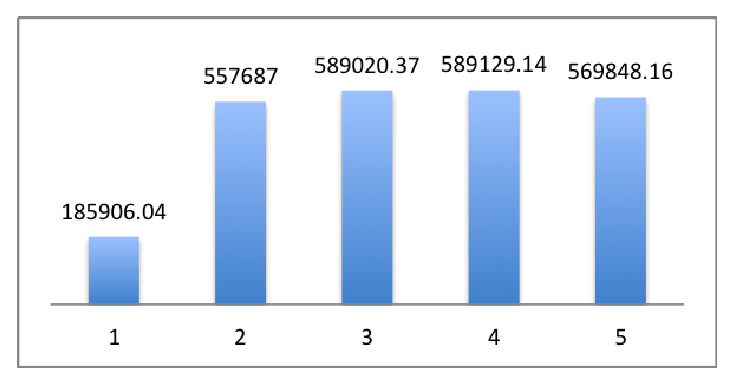
\includegraphics{perf_ngramlen1-5_distinct-items_supp10+_1hr.eps}}
\rput(18.89,0.5441601){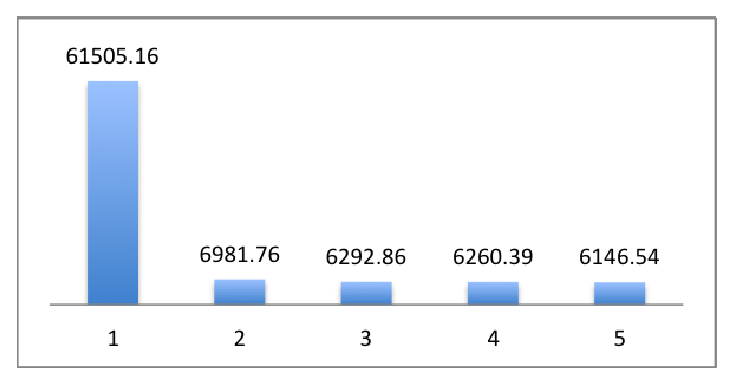
\includegraphics{perf_ngramlen1-5_itemsets_supp10+_1hr.eps}}
\rput(31.89,0.50416017){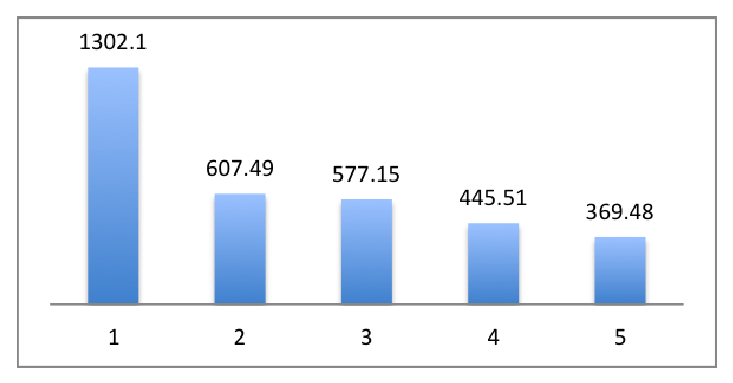
\includegraphics{perf_ngramlen1-5_runtime-millis_supp10+_1hr.eps}}
\end{pspicture} 
}
\caption{Effect of the maximum N-Gram length on the mining of 1hr epochs of data}
\label{fig:ngramsLen}
\end{figure*}

After mining term N-Grams we flatten the itemsets to sets of unigrams again. This removes overlap between parts of  itemsets making it easier to reason about how they relate to each other. This also avoids the possibility that an itemset might be represented differently at different epochs. Actually, within one epoch an itemset will be represented as different N-Gram sets, and we merge them during flattening by taking the union of the posting lists of all the N-Gram sets flattened to the same itemset.

%After flattening, we remove one more type of uninteresting itemsets produced just because the definition of closed itemsets cover it - the empty itemset and individual unigrams. In the rest of this paper we exclude them altogether, so an itemset  simply by not producing an itemset whose length is less than 2.


\section{Temporal mining}
\label{sec:KLD}
KL-Divergence 

\section{Strongly closed itemsets alliances}
\label{sec:strong}
The closed property of an itemset is very easily violated by modifying one document that contains the itemset and removing one of its items. While an update operation is not supported in the model of frequent itemsets mining, a similar effect happens when people are writing about a certain fine grained topic. For example, on November 9th, 2012 many people where tweeting that "Justin Bieber and Selena Gomez broke up". If all Tweets which use the verb "break up" to report the topic also contain the two names in full, then there will be one closed itemset with all 6 items. However, a Tweet can contain any of 8 other combinations of the four names that fully convey the meaning. We can consider that Tweets with any of these combinations are modifications of the \emph{maximal} closed itemset. Therefore instead of 1 maximal itemset about the topic there will be 9 closed ones. Now consider that it is possible to say that "Justin and Selena broke up" as well as "Justin broke up with Selena", resulting in 2 maximal itemsets. This increase in the number of maximal itemsets because of slight variations in the language is intensified by the length limit on Tweets, specially when people try to make space for their comment about a Tweet they are retweeting. We therefore need a property between the easily violated closed property and the very strict maximal property which also results in a large number of redundant itemsets. 
% This will result in the creation of two closed itemsets, a new shorter with support that one higher than the original itemset

We define a \emph{strongly closed} itemset as a closed itemset whose frequency comprises more than a certain proportion of the frequency of its least frequent subset, or which has at least one strongly closed superset. This property chooses closed itemsets which violate the closed property of their subsets by a significant amount. It also filters out itemsets that are short language constructs, because they appear very frequently and none of their numerous supersets comprise a significant proportion of their high frequency. Notice that within the documents containing a closed itemset, $D_{itemset}$, the probability of a closed superset ($\|D_{superset}\| / \|D_{itemset}\|$) is called the confidence of the rule ``$itemset \rightarrow superset$.'' This property is the basic property used for association rules mining, and some algorithms for mining itemsets based on a variation called \emph{all confidence} have been proposed \cite{confidenceclosed}. The strongly closed property builds on the notion of confidence by choosing itemsets which would result in rules of high confidence. The minimum acceptable confidence of the resulting rule is a parameter $\kappa$ that can vary between 0 and 1 to increase the strength of the strongly closed property.

%Using a lower bound on confidence of a longer itemset given a closed subset its least frequent closed subset (maximum confidence of this superset) 
Even though choosing strongly closed itemsets filters out many redundant itemsets formed because of slight variations of the same topic, it is still not a strong enough property. The intersection of the sets of documents containing two strongly closed itemsets can be different by only 1 document from either of the sets. For example, the closed itemset \{justin, selena\} can have three closed supersets: \{justin, selena, broke, up, \#jelena\}, \{justin, selena, broke, up\} and \{justin, selena, \#jelena\}. Figure \ref{fig:jelena} illustrates how all supersets can be strongly closed, while they are still redundant itemsets mined from almost the same documents. Each circle in the figure represents the set of documents containing the superset formed by concatenating the words in the circle with the words in its container. The figure also shows, as dashed circles, examples of itemsets that would be filtered out by the strongly closed property.
\begin{figure}[htb]
\label{fig:jelena}
\centering
% Generated with LaTeXDraw 2.0.8
% Mon Apr 29 15:14:17 EDT 2013
% \usepackage[usenames,dvipsnames]{pstricks}
% \usepackage{epsfig}
% \usepackage{pst-grad} % For gradients
% \usepackage{pst-plot} % For axes
\scalebox{1} % Change this value to rescale the drawing.
{
\begin{pspicture}(0,-1.26)(4.64,1.26)
\psframe[linewidth=0.018,dimen=outer](4.64,1.26)(0.0,-1.26)
\pscircle[linewidth=0.018,dimen=outer](1.48,-0.12){0.94}
\pscircle[linewidth=0.018,dimen=outer](1.96,-0.12){0.9}
\pscircle[linewidth=0.018,linestyle=dashed,dash=0.16cm 0.16cm,dimen=outer](3.81,0.39){0.27}
\usefont{T1}{ptm}{m}{n}
\rput(1.2158496,1.005){Justin, Selena}
\usefont{T1}{ptm}{m}{n}
\rput(1.324287,-0.295){broke, up}
\usefont{T1}{ptm}{m}{n}
\rput(2.2092774,0.125){\#jelena}
\usefont{T1}{ptm}{m}{n}
\rput(3.655244,0.825){Drew}
\pscircle[linewidth=0.018,linestyle=dashed,dash=0.16cm 0.16cm,dimen=outer](3.83,-0.47){0.29}
\usefont{T1}{ptm}{m}{n}
\rput(3.6618066,-0.875){Marie}
\end{pspicture} 
}
\caption{Strongly and not strongly closed itemsets}
\end{figure}

To remove such redundancy, we merge strongly closed itemsets with high cosine similarity into an itemset \emph{alliance}. The itemset alliance is a bag of items formed by taking the union of all member itemsets. This concentrates the numerous  itemsets about a certain topic into one unit. The alliance also include itemsets that are not supersets of one another; for example, itemsets that differ because of items that come earlier in the total ordering and are not pertaining to the topic, such as ``with'' and ``and'' in the Justin-Selena example. The use of cosine similarity limits the candidates for merging to itemsets that are very likely about the same topic, since the Inverse Document Frequency (IDF) value of terms pertaining to a certain topics is typically much higher than the IDF value of other terms. The IDF and cosine similarity formulae used are given in equations \ref{eq:IDF} and \ref{eq:cosine} respectively.

\begin{equation}\label{eq:IDF}IDF(i) = \log{\frac{\|E\|}{\|D_i\|}}\end{equation}

\begin{equation}\label{eq:cosine}cos(S_1,S_2) = \frac{\sqrt{\sum_{i \in S_1 \cap S_2} IDF(i)^2 }}{\sqrt{\sum_{i \in S_1} IDF(i)^2} * \sqrt{\sum_{i \in S_2} IDF(i)^2}} \end{equation}

To avoid forming alliances that are not coherent about a certain topic, we calculate the difference between the posting lists of every two itemsets being merged. The merge is permitted only if the difference is below the maximum number of different document allowed for the required closed strength, given by equation \ref{eq:maxDiffCnt}. In case of merging an itemset with its superset, this difference can be calculated directly from the sizes of the posting lists.
% using the confidence formula.
%by subtracting the support of the superset from that of the itemset. 
Otherwise, the difference can be efficiently calculated from the postings lists since they are sorted, and in fact it is enough to check if the difference exceeds the maximum number allowed.
% The maximum number of different documents is given by equation \ref{eq:maxDiffCnt}. 
%An empirical performance evaluation is provided in section \ref{sec:perf}. 

\begin{equation}\label{eq:maxDiffCnt}\Delta(S_1,S_2,\kappa) = (1 - \kappa) * max(\|D_{S_1}\|,\|D_{S_2}\|), \, \kappa \in [0,1[\end{equation}

After joining an alliance an itemset seizes to exist outside of the alliance, so that an itemset can be part of only one alliance. However, when checking which itemsets to consider for merging with a still unallied itemset, its similarity is calculated with the individual itemsets rather than the alliance. Otherwise, an itemset could fail to join an existing alliance because the similarity between the larger bag of items and the itemset is likely to be lower than the similarity between individual member itemsets and the itemset. This can cause cascading many alliances that should have been separate into one large alliance. Such an oversized alliance could also be about different topics. Empirically, we observe that one and only one oversized alliance about different topics is formed. This alliance catches many itemsets made up of low IDF terms, thus not interesting. Topics with high IDF terms in them cannot have high cosine similarity with topics of only low IDF terms. The size of the bag of items in this alliance is significantly larger than other alliances, making it easy to distinguish and discard it.
%It is difficult to reason about how alliances are formed, specially after fi

%Expanding on the previous observation that adding a high IDF term to an itemset with low IDF terms only prevents achieving a high enough cosine similarity, we introduce an optimization that improves both runtime, memory requirements and filtering power. Unlike the original LCM algorithm, our extension requires keeping previous itemsets in memory so that newly generated ones are compared to them to find candidates for alliance. Instead of keeping all previous itemsets in memory we keep only a limited number, $b$. This obviously improves runtime and memory requirements, but it also improves the quality of itemsets chosen for alliance. Given the way PPC-Extension produces itemsets, an alliance candidate appearing more than $b$ itemsets earlier must be similar because of a term that has at least $\log_2(b+1)$  extension items \emph{smaller} than the one that got added to form the current itemset. This lower bound assumes that all possible itemsets created by appending any combination of the $\log_2(b+1)$ will be closed and will have enough support. In this case, there will be 1 combination where all the items are appended, $\log_2(b+1)$ combinations where one item is missing, $\log_2(b+1)$ choose 2 combinations where 2 items are missing, ... etc. For all of these combinations to be closed itemsets, the 1 combination where all the items are appended has to have minimum support, the  $\log_2(b+1)$ combinations where 1 item is missing will each have support 1 more than minimum, the combinations where 2 items are missing will each have support 2 more than minimum, ... etc. Therefore the minimum drop in frequency between a closed itemsets and its subset produced $b$ steps earlier is given by:
%\begin{equation}\|D_{S_x}\| - \|D_{S_(x-b)}\| = \alpha \|E\| + \sum_{a=1}^{\log_2(b+1) - 1}a\binom{\log_2(b+1)}{a} \end{equation}
%To minimize the difference in frequency between the current itemset and the alliance candidate, we assume that the 1 combination will appear $\ciel{b/2}$ times,  Therefore the difference in frequency between  $b$ 


Expanding on the previous observation that adding a high IDF term to an itemset with low IDF terms only prevents achieving a high enough cosine similarity, we introduce an optimization that improves both runtime, memory requirements and filtering power. Unlike the original LCM algorithm, our extension requires keeping previous itemsets in memory so that newly generated ones are compared to them to find candidates for alliance. Instead of keeping all previous itemsets in memory we keep only a limited number, $b$. This obviously improves runtime and memory requirements, and it can also improve the quality of itemsets chosen for alliance. If the total ordering follows the descending order of items' frequencies, then, because of the way PPC-Extension produces itemsets, for an itemset $S_x$ and any candidate subset $S_{(x-b)}$ that was produced $b$ itemsets earlier $\|D_{S_{(x-b)}}\| - \|D_{S_x}\| \ge b$. This lower bound is achieved when the intersection of the documents containing the current itemset $S_x$ and all the $b-1$ supersets before it is exactly the subset $S_{(x-b)}$, and there are no more itemsets with the same intersection. In this case each of the $b$ supersets must have support at most $\|D_{S_{(x-b)}}\| - 1$ to be considered closed, but because there are $b$ of them then actually their support is $\|D_{S_{(x-b)}}\| - b$. Since the minimum support difference is $b$, then the maximum confidence of $S_x$ is $\frac{\|D_{S_{(x-b)}}\| - b}{\|D_{S_{(x-b)}}\|} $. Therefore for a given $\kappa$ we can determine the buffer size $b$ as the frequency of itemsets keeps decreasing. In our implementation we use a fixed $b$ of 1000.

%A similar situation also happens if the intersection ???
%must have a frequency of occurrence at least $b$ more than the current itemset's frequency. 

Algorithm \ref{algo:alliance} shows the described algorithm for merging itemsets alliances. Table  \ref{table:allianceQuality} shows the number of closed itemsets of length at least 2 without filtering any of them out, as well as after applying the KLD filter and the strongly closed filter, and the number of itemsets alliances. The table also shows the average quality of the itemsets after each stage of reduction. The quality is calculated as Basic Elements? PERPLEXITY? CASCADE MEASURE? 

\begin{algorithm}
\SetAlgoLined
\LinesNumbered
\KwIn{$\theta$: Minimum cosine similarity, \\$\kappa$: Minimum closed strength}
\KwData{S: Frequent Itemsets produced by LCM}
\KwResult{A: Frequent Itemsets alliances}
\For{$i \gets 2$ to $\|S\|$}{
	$C \gets \emptyset$ \tcp*{Candidates for merging with $S_i$}
	$T \gets \emptyset$ \tcp*{Subsets of current itemset}
	\For{$j \gets 1$ to $i - 1$}{
		\uIf{$\|S_i \cap S_j\| = min(\|S_i\|, \|S_j\|)$}{
			$C$.add($S_j$)\;
			\lIf{$\|S_i\| > \|S_j\|$}{$T$.add($S_j$)}
		}
		\ElseIf{cos($S_i,S_j$) $\ge \theta$}{
			$C$.add($S_j$)\;
		}
	}
	$M.score \gets \infty$ \tcp*{Best merge candidate's score}
	\ForEach{$S_c \in C$}{
		\uIf{$S_c \in T$}{
			$\delta \gets \|D_{S_c}\| - \|D_{S_i}\|$\;
		}	
		\Else{
			$\delta \gets$ difference($D_{S_i},D_{S_c}$) \tcp*{Stops early}
		}
		\If{$\delta \le \Delta(S_i, S_c, \kappa)$ and $\delta < M.score$}{
			$M \gets S_c$\;
			$M.score \gets \delta$\;
		}
	}
	\If{$M.score < \infty$}{
		A[M].$itemset \gets $A[M].$itemset \cup S_i \cup M$\;
	}
}
\Return{A}\;
\caption{Merging itemsets into alliances}
\label{algo:alliance}
\end{algorithm}



% The difference between documents containing a certain strongly closed itemset and the intersection can be as little as one document. Thus all variations can have high confidence. On the other hand, using an upper bound on confidence is totally counter intuitive, since this means that if only one document exists with a shorter itemset then the longer itemset will be omitted. 
%Observe that all documents containing the longer itemset will also contain the shorter itemset, and it is possible for several variations to have high confidence because documents
%filters out many redundant closed itemsets, but cannot filter out formed because of slight variations of the same topic. 

%We build on the confidence property by merging high confidence itemsets that are extensions of the same itemset into an itemset \emph{alliance}. The itemset alliance is a bag of items formed by taking the union of all member itemsets. This concentrates the numerous high confidence closed and maximal itemsets about a certain topic into one unit. Furthermore, we also include in the alliance all itemsets with high cosine similarity to its members. This merges together itemsets that differ because of items that come earlier in the total ordering and are not pertaining to the topic, such as ``with'' and ``and'' in the Bieber-Gomez example. To avoid forming alliances that are not coherent about a certain topic, we go beyond the numerical calculation of confidence and we actually calculate the overlap between the posting lists of itemsets being merged. In case of merging an itemset with its subset 
%With a reasonably high support, the 
 


\section{Empirical Evaluation}
\label{sec:empirical}
Examples from Nov. 6 and 9. Nov. 9 has two events for Bieber.. MTVEMA and break up.

\section{Related work}
\label{sec:related}

\section{Conclusion and future work}
\label{sec:concfut}

\section{Acknowledgement}

%
% The following two commands are all you need in the
% initial runs of your .tex file to
% produce the bibliography for the citations in your paper.
%\bibliographystyle{abbrv}
%\bibliography{sigproc}  % sigproc.bib is the name of the Bibliography in this case
% You must have a proper ".bib" file
%  and remember to run:
% latex bibtex latex latex
% to resolve all references
%
% ACM needs 'a single self-contained file'!
%
%APPENDICES are optional
%\balancecolumns

\end{document}
